\documentclass[10pt,aspectratio=169]{beamer}

\usepackage[spanish,es-nodecimaldot]{babel}
\usepackage[utf8]{inputenc}
\usepackage[T1]{fontenc}
\usepackage{lmodern}
\usepackage{booktabs}
\usepackage{graphicx}
\usepackage{amsmath}
\usepackage{tikz}
\usetikzlibrary{arrows.meta,positioning}
\usepackage{hyperref}

\usetheme{Madrid}
\usecolortheme{seahorse}
\definecolor{uvblue}{HTML}{12406B}
\setbeamercolor{structure}{fg=uvblue}
\setbeamercolor{title}{fg=white,bg=uvblue}
\setbeamercolor{frametitle}{fg=white,bg=uvblue}
\setbeamertemplate{navigation symbols}{}
\setbeamertemplate{caption}[numbered]
\setbeamerfont{caption}{size=\scriptsize}
\setbeamerfont{frametitle}{size=\large}

% Archivo generado automáticamente por src/build_docs.py. No editar a mano.
\newcommand{\Accuracy}{0.6771}
\newcommand{\MacroPrecision}{0.6786}
\newcommand{\MacroRecall}{0.6655}
\newcommand{\MacroF}{0.6663}
\newcommand{\WeightedF}{0.6762}
\newcommand{\TopThree}{0.8452}
\newcommand{\BestValAcc}{0.7491}
\newcommand{\ValTestGap}{7.20}
\newcommand{\EpochsRun}{8}
\newcommand{\BestEpoch}{3}
\newcommand{\NumParams}{5.13}
\newcommand{\ParamsExact}{5{,}125{,}396}
\newcommand{\TrainTime}{27.9}
\newcommand{\TrainTimeMin}{0.5}
\newcommand{\Vocab}{20{,}000}
\newcommand{\NTrain}{10{,}182}
\newcommand{\NVal}{1{,}132}
\newcommand{\NTest}{7{,}532}
\newcommand{\NTrainTotal}{11{,}314}
\newcommand{\NTestTotal}{7{,}532}
\newcommand{\WordsMean}{185.8}
\newcommand{\WordsMedian}{83}
\newcommand{\WordsPNoventaCinco}{572}
\newcommand{\WordsMax}{11{,}765}
\newcommand{\EmptyDocs}{300}
\newcommand{\Imbalance}{1.59}
\newcommand{\MaxClassName}{rec.sport.hockey}
\newcommand{\MaxClassCount}{600}
\newcommand{\MinClassName}{talk.religion.misc}
\newcommand{\MinClassCount}{377}
\newcommand{\NumExperiments}{9}
\newcommand{\PrimaryName}{MLP 1$\times$256 (principal)}
\newcommand{\BestName}{MLP 1$\times$256 (principal)}
\newcommand{\BestAcc}{0.6771}
\newcommand{\BestF}{0.6663}
\newcommand{\LinearAcc}{0.6572}
\newcommand{\LinearF}{0.6451}
\newcommand{\OneHiddenAcc}{0.6771}
\newcommand{\OneHiddenF}{0.6663}
\newcommand{\DropoutAcc}{0.6644}
\newcommand{\DropoutF}{0.6566}
\newcommand{\DropoutEpochs}{9}
\newcommand{\DropoutParams}{10.4M}
\newcommand{\DeepAcc}{0.6498}
\newcommand{\DeepF}{0.6433}
\newcommand{\DeepEpochs}{13}
\newcommand{\DeepParams}{10.4M}
\newcommand{\VocabTenAcc}{0.6439}
\newcommand{\VocabTenF}{0.6358}
\newcommand{\VocabTenEpochs}{11}
\newcommand{\VocabTenParams}{5.3M}
\newcommand{\BalancedAcc}{0.6686}
\newcommand{\BalancedF}{0.6568}
\newcommand{\BalancedEpochs}{8}
\newcommand{\BalancedParams}{10.4M}
\newcommand{\LrAcc}{0.6741}
\newcommand{\LrF}{0.6653}
\newcommand{\LrEpochs}{10}
\newcommand{\LrParams}{10.4M}
\newcommand{\LtwoAcc}{0.6455}
\newcommand{\LtwoF}{0.6393}
\newcommand{\LtwoEpochs}{12}
\newcommand{\LtwoParams}{10.4M}
\newcommand{\LinearEpochs}{11}
\newcommand{\LinearParams}{0.4M}
\newcommand{\OneHiddenEpochs}{8}
\newcommand{\OneHiddenParams}{5.1M}
\newcommand{\PrimaryParams}{5.1M}
\newcommand{\TwoLayerAcc}{0.6680}
\newcommand{\TwoLayerF}{0.6578}
\newcommand{\TwoLayerEpochs}{10}
\newcommand{\TwoLayerParams}{10.4M}

\graphicspath{{../results/figures/}}

\title[MLP para clasificación de texto]{Perceptrón Multicapa para clasificación de texto}
\subtitle{20 Newsgroups con Keras/TensorFlow --- Entrega 1}
\author[Redes Neuronales]{Nicolás Garcés (218066) \and Juan Pablo Ante (2140132)}
\institute[Univalle]{Escuela de Ingeniería de Sistemas y Computación\\Universidad del Valle}
\date{2026-2}

\begin{document}

% ----------------------------------------------------------------------
\begin{frame}
  \titlepage
\end{frame}

% ----------------------------------------------------------------------
\begin{frame}{Problema y objetivos}
  \begin{columns}[T]
    \begin{column}{0.55\textwidth}
      \textbf{Problema.} Clasificar mensajes de Usenet en 20 categorías
      temáticas a partir de su texto.
      \vspace{0.3cm}

      \textbf{Por qué es difícil.}
      \begin{itemize}
        \item Texto disperso, ruidoso y de longitud variable.
        \item Clases temáticamente solapadas (computación, religión, política).
        \item Metadatos con fuga de información si no se eliminan.
      \end{itemize}
    \end{column}
    \begin{column}{0.42\textwidth}
      \begin{block}{Objetivo}
        Entrenar y evaluar una \textbf{MLP} en Keras/TensorFlow, ajustar sus
        hiperparámetros y analizar críticamente sus errores.
      \end{block}
      \begin{alertblock}{Alcance}
        Clasificación \textbf{multiclase} (una etiqueta por documento), tal
        como están anotados los datos.
      \end{alertblock}
    \end{column}
  \end{columns}
\end{frame}

% ----------------------------------------------------------------------
\begin{frame}{Conjunto de datos: 20 Newsgroups}
  \begin{columns}[T]
    \begin{column}{0.48\textwidth}
      \begin{table}
        \centering
        \small
        \begin{tabular}{lr}
          \toprule
          Documentos de entrenamiento & \NTrainTotal \\
          Documentos de prueba & \NTestTotal \\
          Clases & 20 \\
          Palabras por documento (media) & \WordsMean \\
          Palabras por documento (mediana) & \WordsMedian \\
          Desbalance (mayor/menor) & \Imbalance$\times$ \\
          \bottomrule
        \end{tabular}
      \end{table}
      \vspace{0.1cm}
      \small
      Partición oficial de scikit-learn. Se eliminan \textbf{cabeceras, pies
      y citas} para evitar que el nombre del grupo revele la etiqueta.
    \end{column}
    \begin{column}{0.50\textwidth}
      \centering
      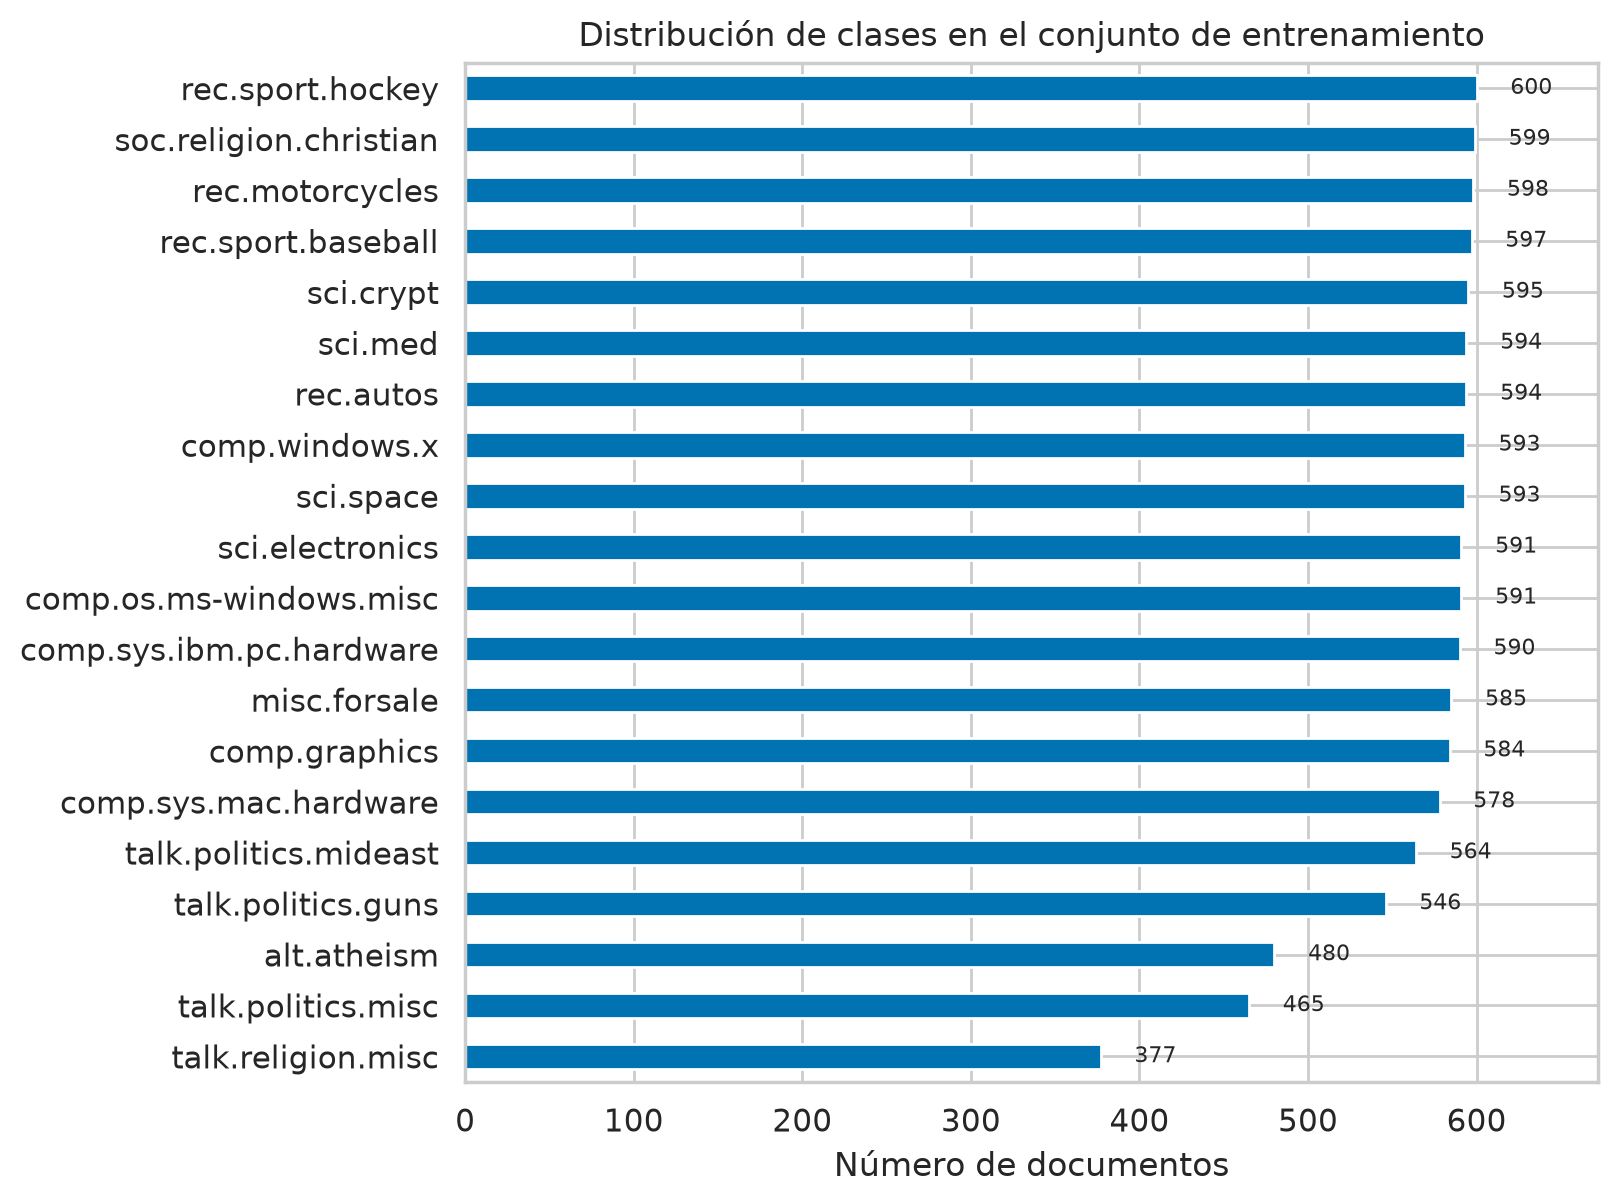
\includegraphics[width=\textwidth]{eda_distribucion_clases.png}
    \end{column}
  \end{columns}
\end{frame}

% ----------------------------------------------------------------------
\begin{frame}{Preprocesamiento y protocolo}
  \begin{enumerate}
    \item \textbf{Texto crudo}: minúsculas, sin puntuación, tokenización por espacios.
    \item \textbf{TF-IDF} con vocabulario de \Vocab{} términos, adaptado
          \alert{solo con entrenamiento}.
    \item \textbf{Partición}: 90\,\% train / 10\,\% validación (estratificada);
          prueba oficial intacta hasta el final.
    \item \textbf{Normalización} de cada vector TF-IDF a norma unitaria.
  \end{enumerate}
  \vspace{0.3cm}
  \begin{block}{Por qué TF-IDF}
    Señal densa y discriminativa, entrenamiento rápido y línea base fuerte.
    Para una MLP pura es más estable que embeddings aprendidos desde cero.
  \end{block}
\end{frame}

% ----------------------------------------------------------------------
\begin{frame}{Arquitectura}
  \centering
  \begin{tikzpicture}[
    node distance=0.65cm and 0.55cm,
    box/.style={draw=uvblue, fill=blue!8, rounded corners=3pt, align=center,
                minimum height=1.3cm, minimum width=2.3cm, font=\small},
    arrow/.style={-{Latex[length=2.4mm]}, thick, draw=black!60}
  ]
    \node[box] (texto) {Texto\\crudo};
    \node[box, right=of texto] (tfidf) {TF-IDF\\\Vocab{} términos};
    \node[box, right=of tfidf] (d1) {Dense 256\\ReLU + Dropout 0.3};
    \node[box, right=of d1] (out) {Softmax\\20 clases};
    \draw[arrow] (texto) -- (tfidf);
    \draw[arrow] (tfidf) -- (d1);
    \draw[arrow] (d1) -- (out);
  \end{tikzpicture}
  \vspace{0.5cm}

  \begin{columns}[T]
    \begin{column}{0.48\textwidth}
      \small
      \textbf{\ParamsExact{} parámetros entrenables.}\\
      La capa oculta concentra el 99.9\,\% (5.1 M).
    \end{column}
    \begin{column}{0.48\textwidth}
      \small
      Salida softmax + entropía cruzada categórica dispersa.\\
      Dropout para controlar el sobreajuste.
    \end{column}
  \end{columns}
\end{frame}

% ----------------------------------------------------------------------
\begin{frame}{Condiciones de entrenamiento}
  \begin{columns}[T]
    \begin{column}{0.53\textwidth}
      \begin{table}
        \centering
        \small
        \begin{tabular}{ll}
          \toprule
          Optimizador & Adam ($\eta=10^{-3}$) \\
          Pérdida & Entropía cruzada \\
          Batch & 128 \\
          Épocas máximas & 25 \\
          Parada temprana & \texttt{val\_accuracy}, paciencia 5 \\
          Regularización & Dropout 0.3 \\
          Semilla & 42 (determinista) \\
          Hardware & CPU i5-9400F, 6 núcleos \\
          \bottomrule
        \end{tabular}
      \end{table}
    \end{column}
    \begin{column}{0.44\textwidth}
      \begin{block}{Protocolo de comparación}
        \small
        9 configuraciones con la misma partición, semilla y criterio de parada:
        \begin{itemize}
          \item profundidad: 0, 1, 2 y 3 capas ocultas;
          \item dropout 0.3 vs.\ 0.5--0.4 y L2;
          \item vocabulario \Vocab{} vs.\ 10k;
          \item balanceo de clases;
          \item tasa de aprendizaje y L2.
        \end{itemize}
      \end{block}
    \end{column}
  \end{columns}
\end{frame}

% ----------------------------------------------------------------------
\begin{frame}{Ajuste de hiperparámetros}
  \centering
  \scriptsize
  \setlength{\tabcolsep}{3.5pt}
  \begin{tabular}{lcccc}
    \toprule
    Configuración & Paráms. & Épocas & Exactitud & F1 macro \\
    \midrule
    Lineal (sin capas ocultas) & \LinearParams & \LinearEpochs & \LinearAcc & \LinearF \\
    \textbf{MLP 1$\times$256 (principal)} & \OneHiddenParams & \OneHiddenEpochs & \Accuracy & \MacroF \\
    MLP 2$\times$512--256 & \TwoLayerParams & \TwoLayerEpochs & \TwoLayerAcc & \TwoLayerF \\
    MLP 2$\times$512--256, dropout 0.5--0.4 & \DropoutParams & \DropoutEpochs & \DropoutAcc & \DropoutF \\
    MLP 3$\times$512--256--128 & \DeepParams & \DeepEpochs & \DeepAcc & \DeepF \\
    MLP 2$\times$512--256, vocab.\ 10k & \VocabTenParams & \VocabTenEpochs & \VocabTenAcc & \VocabTenF \\
    MLP 2$\times$512--256, balanceado & \BalancedParams & \BalancedEpochs & \BalancedAcc & \BalancedF \\
    MLP 2$\times$512--256, lr $5\times10^{-4}$ & \LrParams & \LrEpochs & \LrAcc & \LrF \\
    MLP 2$\times$512--256, L2 $10^{-4}$ & \LtwoParams & \LtwoEpochs & \LtwoAcc & \LtwoF \\
    \bottomrule
  \end{tabular}
  \vspace{0.25cm}

  \small
  La primera capa oculta aporta la mayor ganancia; una tercera capa sobreajusta.
\end{frame}

% ----------------------------------------------------------------------
\begin{frame}{Resultados del modelo principal}
  \begin{columns}[T]
    \begin{column}{0.42\textwidth}
      \begin{table}
        \centering
        \small
        \begin{tabular}{lc}
          \toprule
          Métrica & Valor \\
          \midrule
          Exactitud & \textbf{\Accuracy} \\
          Precisión macro & \MacroPrecision \\
          Recall macro & \MacroRecall \\
          F1 macro & \textbf{\MacroF} \\
          F1 ponderado & \WeightedF \\
          Exactitud top-3 & \TopThree \\
          \bottomrule
        \end{tabular}
      \end{table}
      \small
      \begin{itemize}
        \item Mejor época: \BestEpoch{} de \EpochsRun.
        \item Validación: \BestValAcc{}.
        \item Brecha val--test: \ValTestGap{} p.p.
      \end{itemize}
    \end{column}
    \begin{column}{0.56\textwidth}
      \centering
      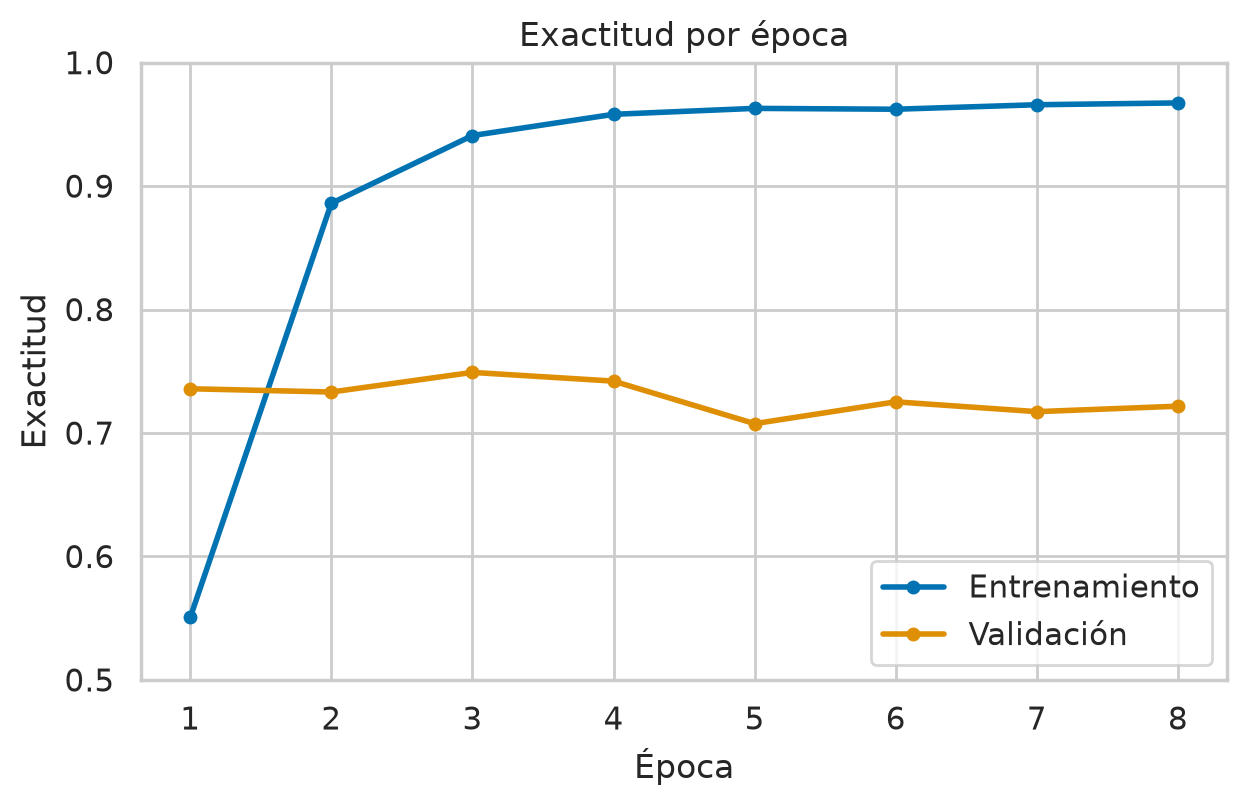
\includegraphics[width=\textwidth]{curvas_exactitud_primary.png}
    \end{column}
  \end{columns}
\end{frame}

% ----------------------------------------------------------------------
\begin{frame}{Matriz de confusión}
  \begin{columns}[T]
    \begin{column}{0.56\textwidth}
      \centering
      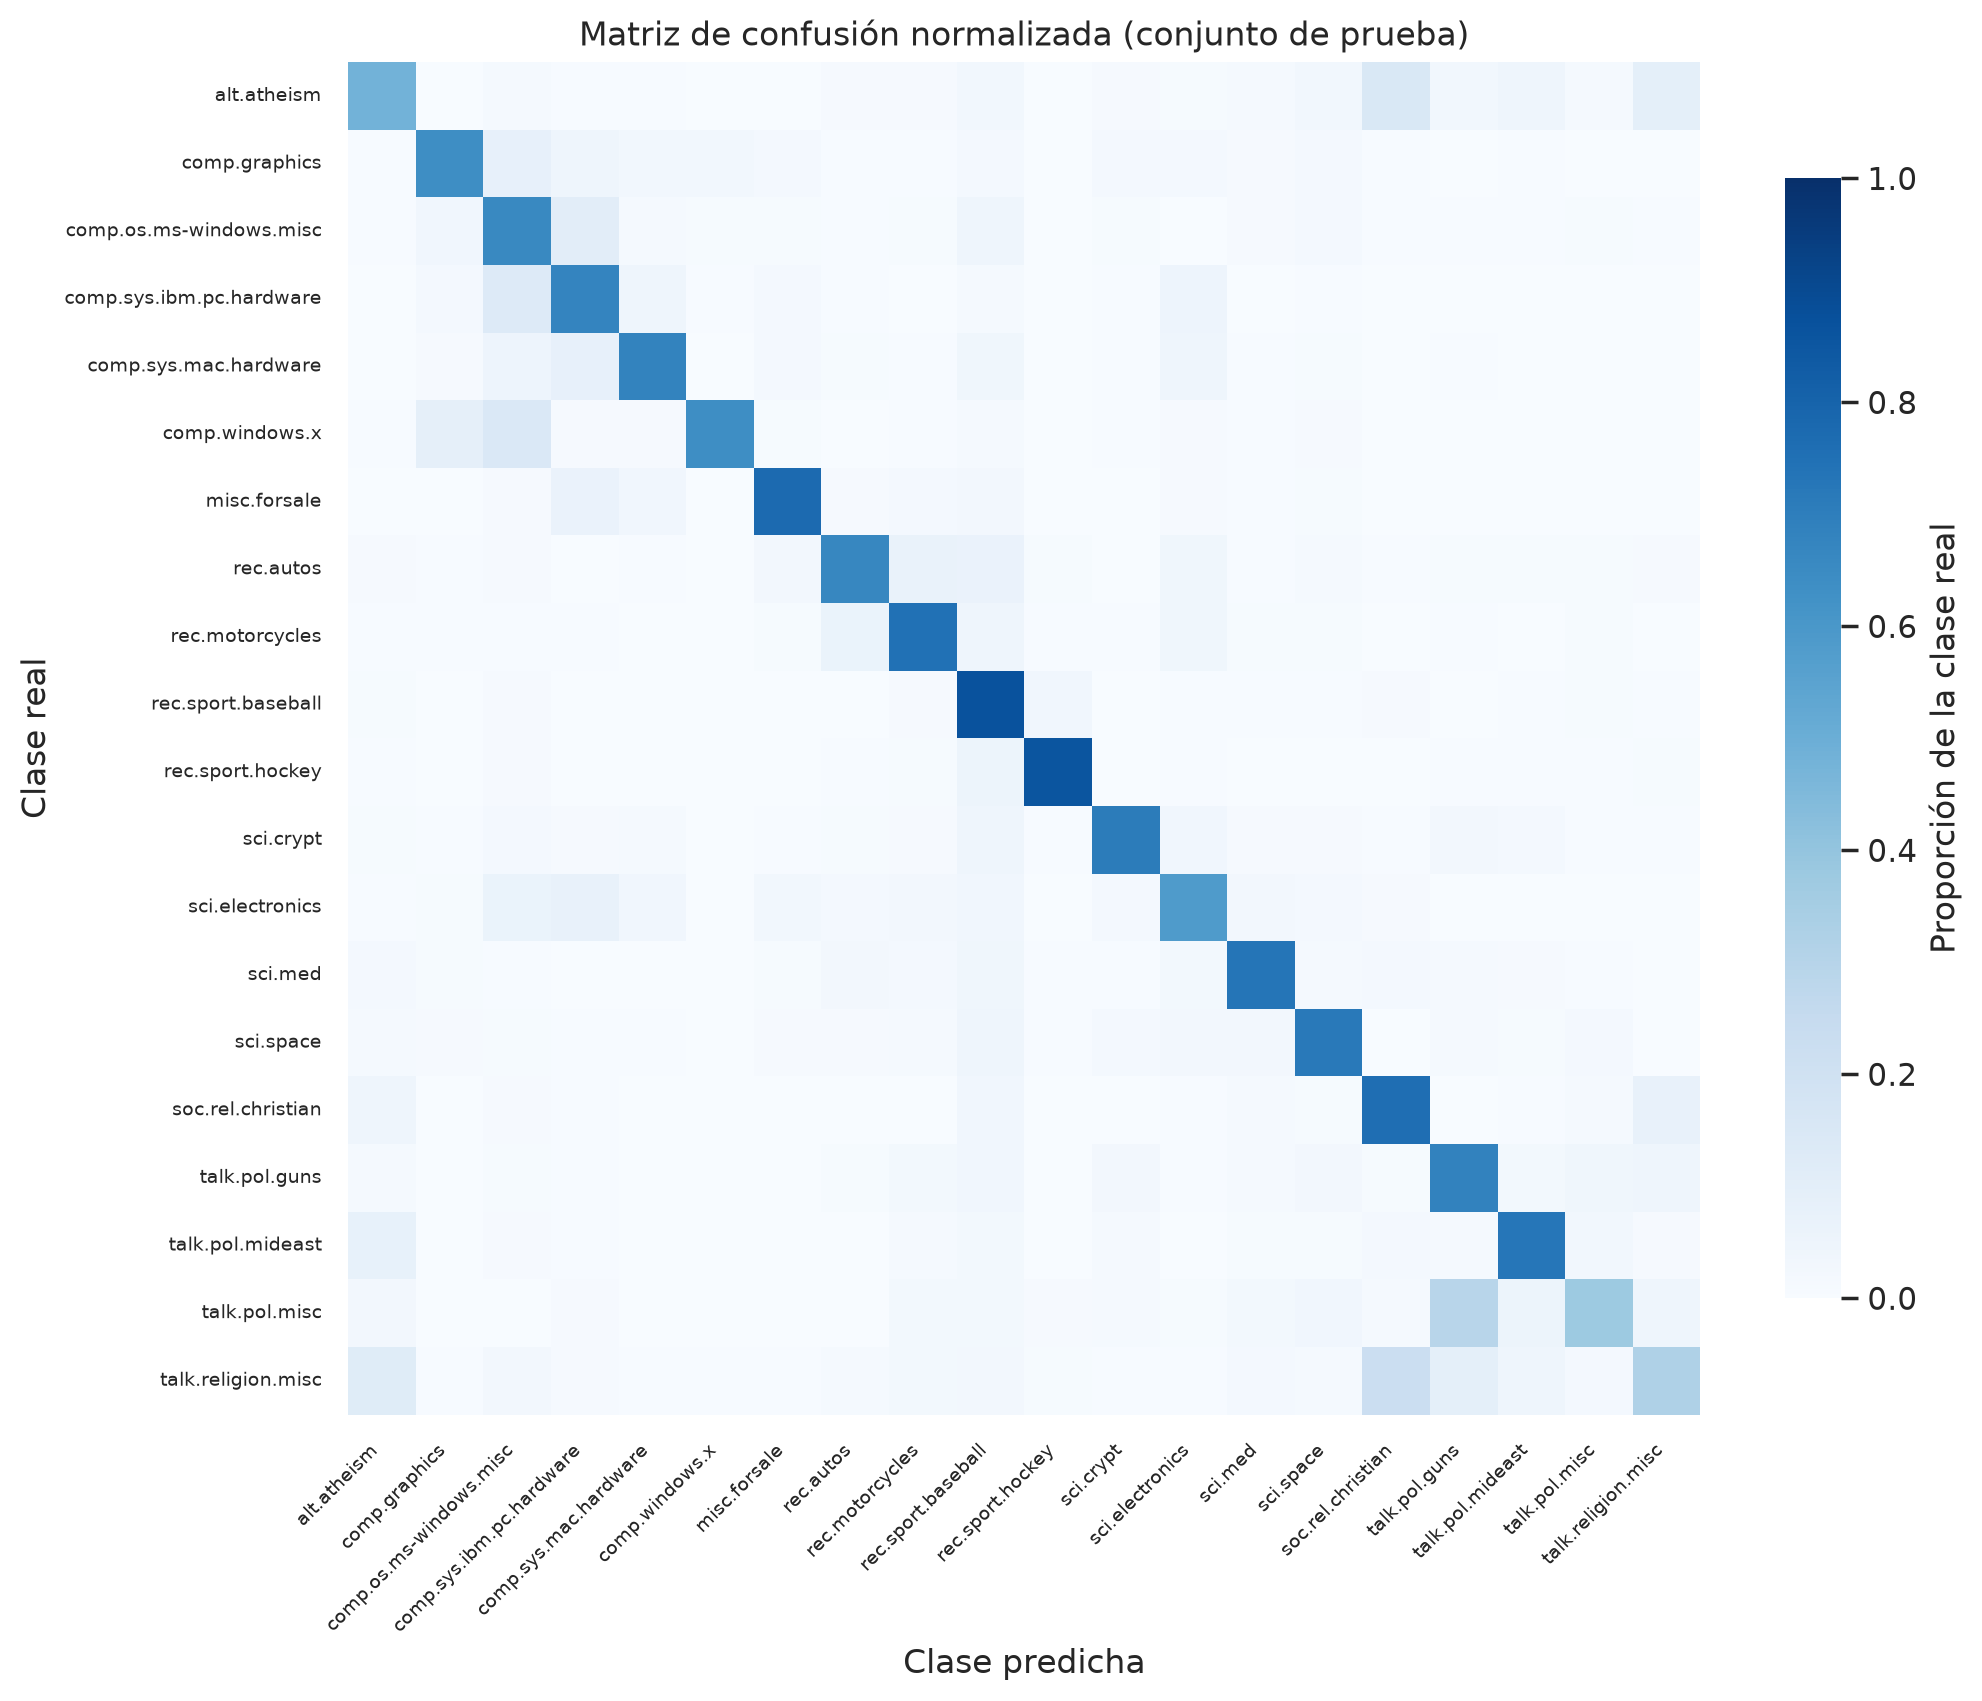
\includegraphics[width=\textwidth]{matriz_confusion_primary.png}
    \end{column}
    \begin{column}{0.42\textwidth}
      \small
      \textbf{Errores estructurados:}
      \begin{itemize}
        \item \texttt{comp.*}: hardware y sistemas operativos comparten vocabulario.
        \item \texttt{alt.atheism}, \texttt{soc.religion.christian} y
              \texttt{talk.religion.misc}: hilos de discusión mezclados.
        \item \texttt{talk.politics.*}: entidades y temas comunes.
      \end{itemize}
      \vspace{0.2cm}
      Los documentos cortos y las respuestas citadas concentran los errores.
    \end{column}
  \end{columns}
\end{frame}

% ----------------------------------------------------------------------
\begin{frame}{Desempeño por clase}
  \begin{columns}[T]
    \begin{column}{0.61\textwidth}
      \centering
      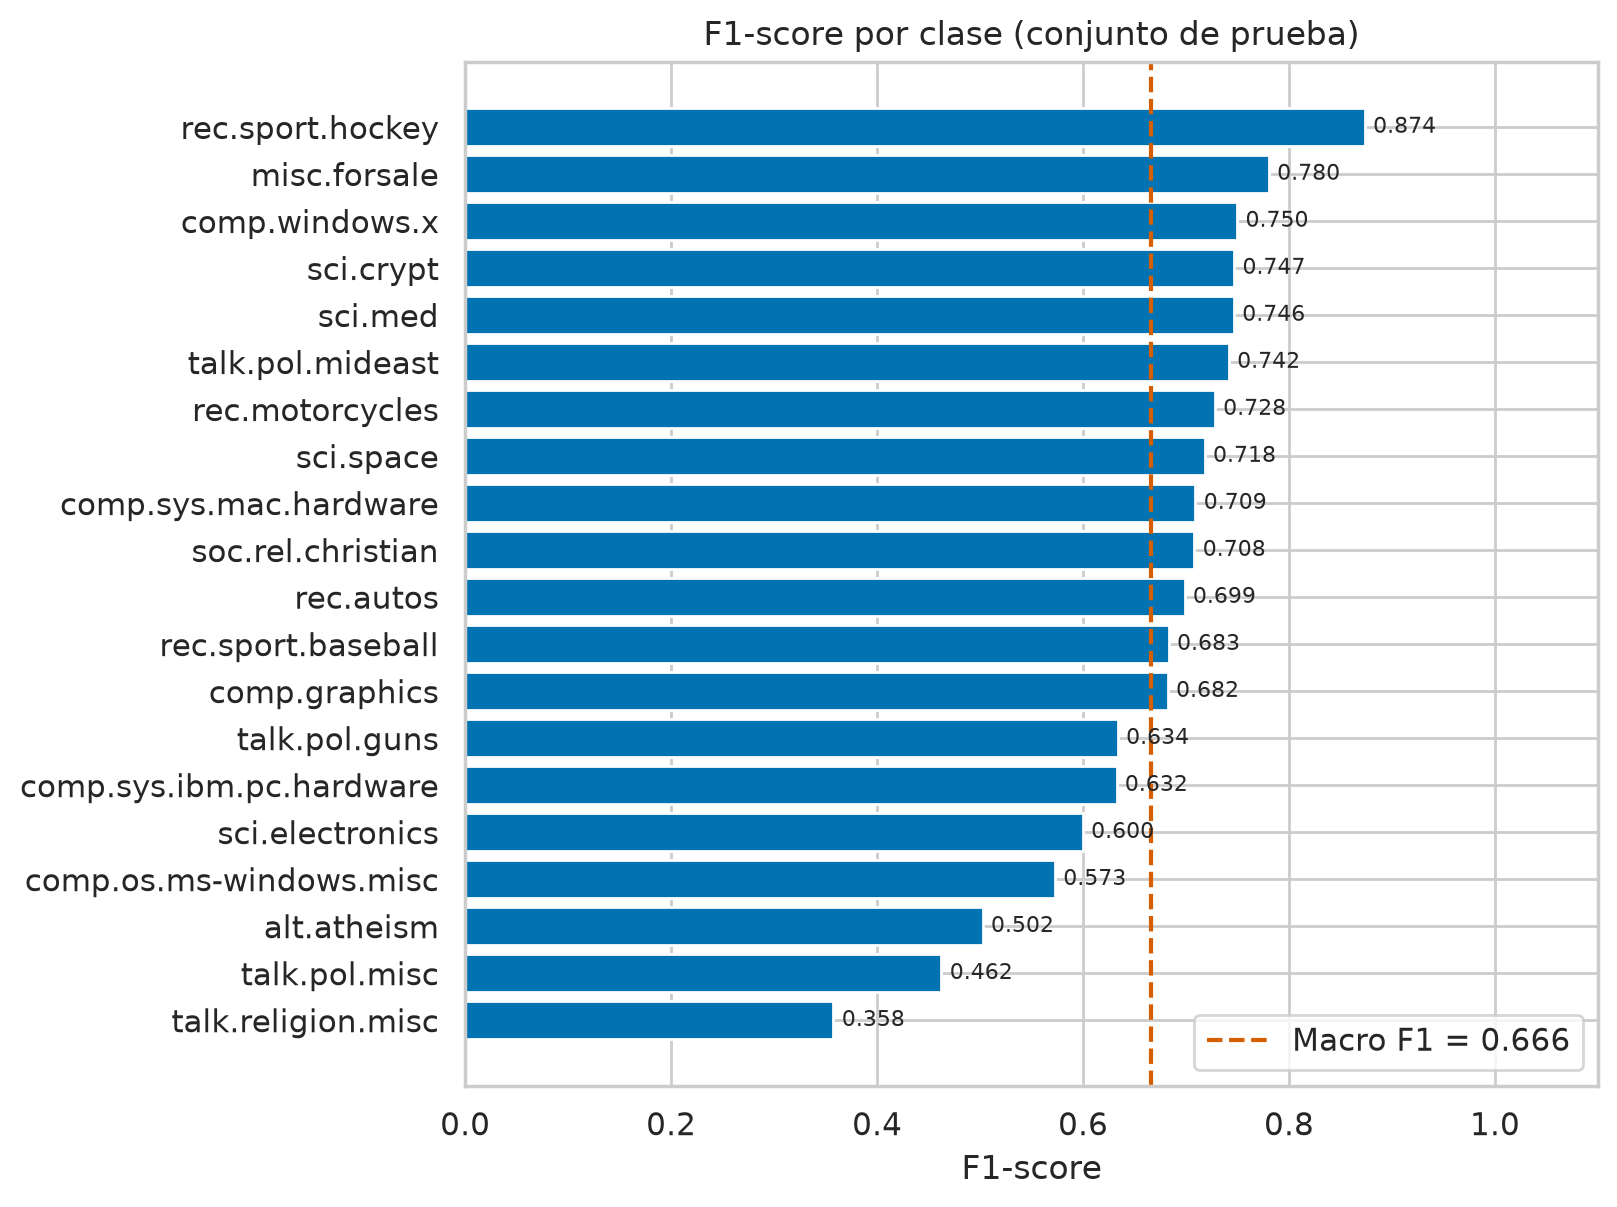
\includegraphics[width=\textwidth]{f1_por_clase_primary.png}
    \end{column}
    \begin{column}{0.37\textwidth}
      \small
      \textbf{Más fáciles}
      \begin{itemize}
        \item \texttt{rec.sport.hockey}: 0.874
        \item \texttt{misc.forsale}: 0.780
        \item \texttt{comp.windows.x}: 0.750
      \end{itemize}
      \textbf{Más difíciles}
      \begin{itemize}
        \item \texttt{talk.religion.misc}: 0.358
        \item \texttt{talk.politics.misc}: 0.462
        \item \texttt{alt.atheism}: 0.502
      \end{itemize}
      \vspace{0.15cm}
      El modelo lineal alcanza \LinearAcc{}; la MLP sube el F1 macro a
      \MacroF{}.
    \end{column}
  \end{columns}
\end{frame}

% ----------------------------------------------------------------------
\begin{frame}{Conclusiones}
  \begin{itemize}
    \item La MLP con TF-IDF alcanza \textbf{\Accuracy{} de exactitud} y
          \textbf{\MacroF{} de F1 macro}, muy por encima del azar.
    \item Una capa oculta de 256 neuronas y dropout 0.3 ofrecen el mejor
          compromiso; añadir capas reduce el F1 macro y el vocabulario
          reducido pierde señal.
    \item El balanceo de clases no compensa la pérdida de exactitud.
    \item Los errores se concentran en clases semánticamente cercanas:
          el modelo no distingue el tema del documento de las palabras citadas.
    \item Limitación: \textit{bag-of-words} ignora orden y contexto.
  \end{itemize}
  \vspace{0.3cm}
  \begin{block}{Siguiente entrega}
    Comparar una RNN sin memoria con una LSTM/GRU o Transformer, capaces de
    modelar secuencia y dependencias de largo plazo.
  \end{block}
\end{frame}

% ----------------------------------------------------------------------
\begin{frame}[fragile]{Demo ejecutable}
  \begin{columns}[T]
    \begin{column}{0.52\textwidth}
      \textbf{Entrenamiento y evaluación}
      \begin{verbatim}
uv venv --python 3.12 .venv
uv pip install -r requirements.txt
.venv/bin/python -m src.experiments
      \end{verbatim}
      \textbf{Predicción interactiva}
      \begin{verbatim}
.venv/bin/python demo.py
.venv/bin/python -m src.predict "texto"
      \end{verbatim}
    \end{column}
    \begin{column}{0.45\textwidth}
      \begin{block}{Salida esperada}
        \small
        \texttt{Predicción: comp.windows.x (0.41)}\\
        \texttt{--- comp.graphics (0.20)}\\
        \texttt{--- comp.os.ms-windows.misc (0.14)}
      \end{block}
      \small
      El notebook \texttt{entrega1\_mlp.ipynb} reproduce el análisis y las
      figuras. Los artefactos quedan en \texttt{results/}.
    \end{column}
  \end{columns}
\end{frame}

% ----------------------------------------------------------------------
\begin{frame}{Bibliografía}
  \footnotesize
  \begin{thebibliography}{9}
    \bibitem{lang1995} K. Lang. NewsWeeder: Learning to Filter Netnews. \textit{ICML}, 1995.
    \bibitem{joachims1998} T. Joachims. Text Categorization with Support Vector Machines. \textit{ECML}, 1998.
    \bibitem{kingma2015} D. P. Kingma, J. Ba. Adam: A Method for Stochastic Optimization. \textit{ICLR}, 2015.
    \bibitem{srivastava2014} N. Srivastava et al. Dropout: A Simple Way to Prevent Neural Networks from Overfitting. \textit{JMLR}, 2014.
    \bibitem{pedregosa2011} F. Pedregosa et al. Scikit-learn: Machine Learning in Python. \textit{JMLR}, 2011.
  \end{thebibliography}
\end{frame}

\end{document}
